\documentclass[11pt, oneside]{article} 	% use "amsart" instead of "article" for AMSLaTeX format
\usepackage{geometry} 		% See geometry.pdf to learn the layout options. There are lots.
\geometry{letterpaper} 		% ... or a4paper or a5paper or ... 
\usepackage[parfill]{parskip} 		% Activate to begin paragraphs with an empty line rather than an indent
\usepackage{graphicx}				% Use pdf, png, jpg, or eps§ with pdflatex; use eps in DVI mode
								% TeX will automatically convert eps --> pdf in pdflatex		
\usepackage{amssymb}
\usepackage{amsmath}
\usepackage{authblk}
\usepackage{framed}
\usepackage[
backend=biber,
style=alphabetic,
]{biblatex}
\usepackage{graphicx}
\graphicspath{ {./images/} }
\usepackage{verbatim}
\usepackage{tikz} 
\usepackage{xcolor,colortbl}
\usepackage{subcaption}
\captionsetup{compatibility=false}
\usepackage{syntonly}

\usepackage[normalem]{ulem}

\title{Spotting Graph Theory Problems in Spot It}
\author[1]{Dave Fetterman}
\author[2]{James Wang}
\affil[1]{Obviously Unemployed}
\affil[2]{Surprisingly Employed}

\date{4/16/23}
\begin{document}
\maketitle

\begin{abstract}

The kids' card game ``Spot It'' supports a unique mechanic: every card of the 55-card deck has eight different symbols, and shares exactly one symbol of some kind with every other card. Intuitively, this seems impossible. The obvious game play (``spot the match'') works for children as young as two; the intricacies of deck construction astound these children of forty-two. In constructing our own deck, we run across interesting problems in graph theory, number theory, and abstract algebra\footnote{There are also representations in projective geometry, but let's save some domains for everyone else.}. Some are solved, some unsolved, but they span a wide range of domains not obviously connected.
\\

\textbf{A deck of $n$ Spot It cards, each featuring $s$ symbols from a catalogue of $m$ total symbol choices can be constructed many ways, but only a few ways if every symbol occurs exactly $g$ times. In that case, the choice of the $(s, g)$ pair both dictates $m$ and $n$ and is strongly restricted.}
\\

However, if $g$ is then of the special form $g=p^k+1, p \in \mathbb{P}, k \in \mathbb{N}$, we can construct a deck with uniform $g$, and beyond that, we can prove the following four constructions are surprisingly equivalent\footnote{Or, at least, one can derive any from another}:
\\
\begin{enumerate}
\item (The Children's Game) A deck of $n$ ``Spot It'' Cards with $s=g$ symbol slots, where each of $m = n$ symbols occurs exactly $g$ times,
\item (Graph Theory) An edge partition of the complete graph $K_n$ into complete subgraphs $K_g$,
\item (Abstract Algebra) A finite (Galois) field of order $g-1$, and
\item (Number Theory) A Perfect Difference Set\cite{1} on $n$ elements.
\end{enumerate} 
 
We then examine other configurations of $s$ and $g$, as well as comment on other reasonable constructions of a ``Spot It'' deck.

\end{abstract}

\section{The Game and the Problem Statement}

Introduced to us by Ari Steinberg, ``Spot It'' is a children's game of 55 cards as shown in Figure~\ref{fig:cards}, featuring eight colorful symbols on each. Though gameplay comes with a few variants in its tiny rulebook, the primary mechanic when presented two cards is \emph{spot the single common symbol first}. The game is simple enough for a two- or three-year old to grasp (and win!), but the question emerges: \emph{just how did they construct such a deck?}\footnote{Note: There have been some other investigations into ``Spot It''\cite{2}, but for the purposes of enjoyment, everything in this paper was researched without reference to \ (Spot It) work.}

\begin{figure}[!htb]
\centering
\begin{subfigure}{.2\textwidth}
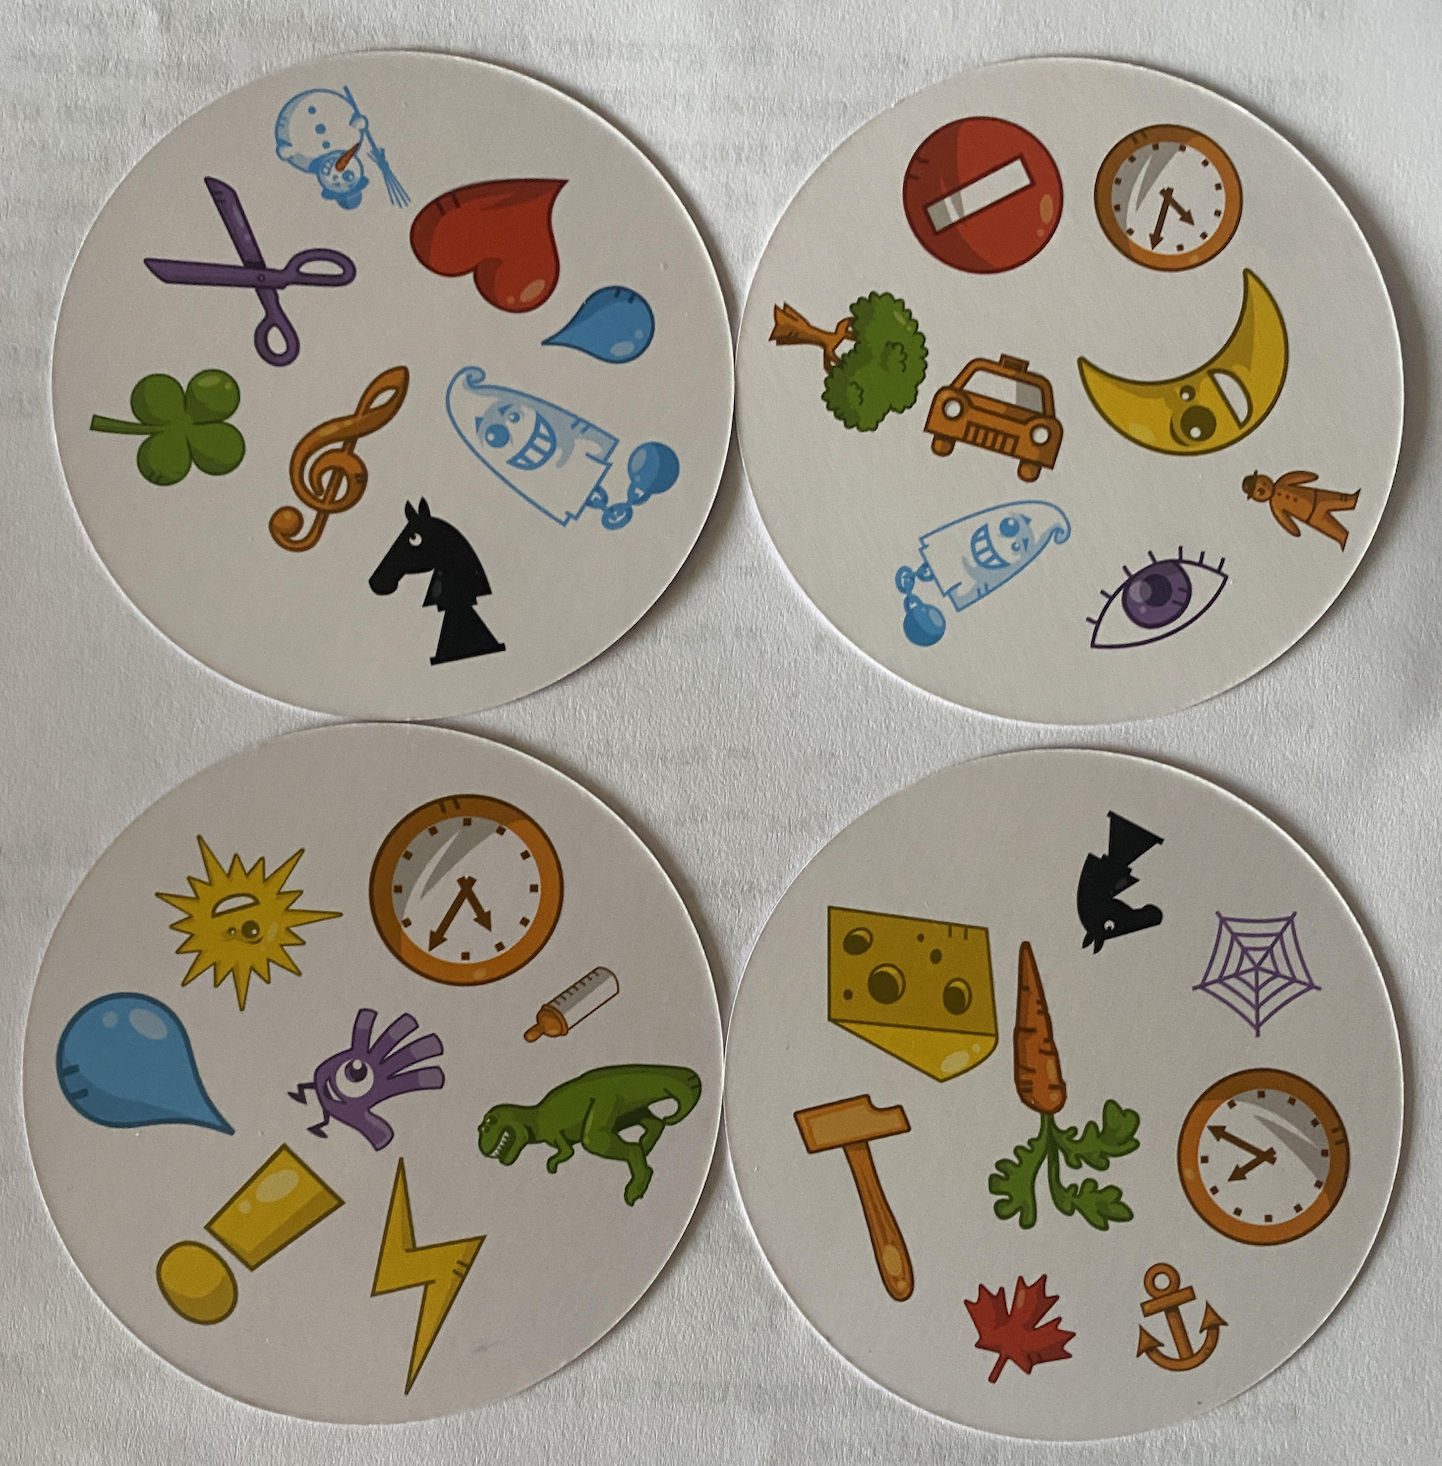
\includegraphics[scale=.2]{cards}
\caption{Four cards in the game}
\label{fig:cards}
\end{subfigure}

\begin{subfigure}{.2\textwidth}
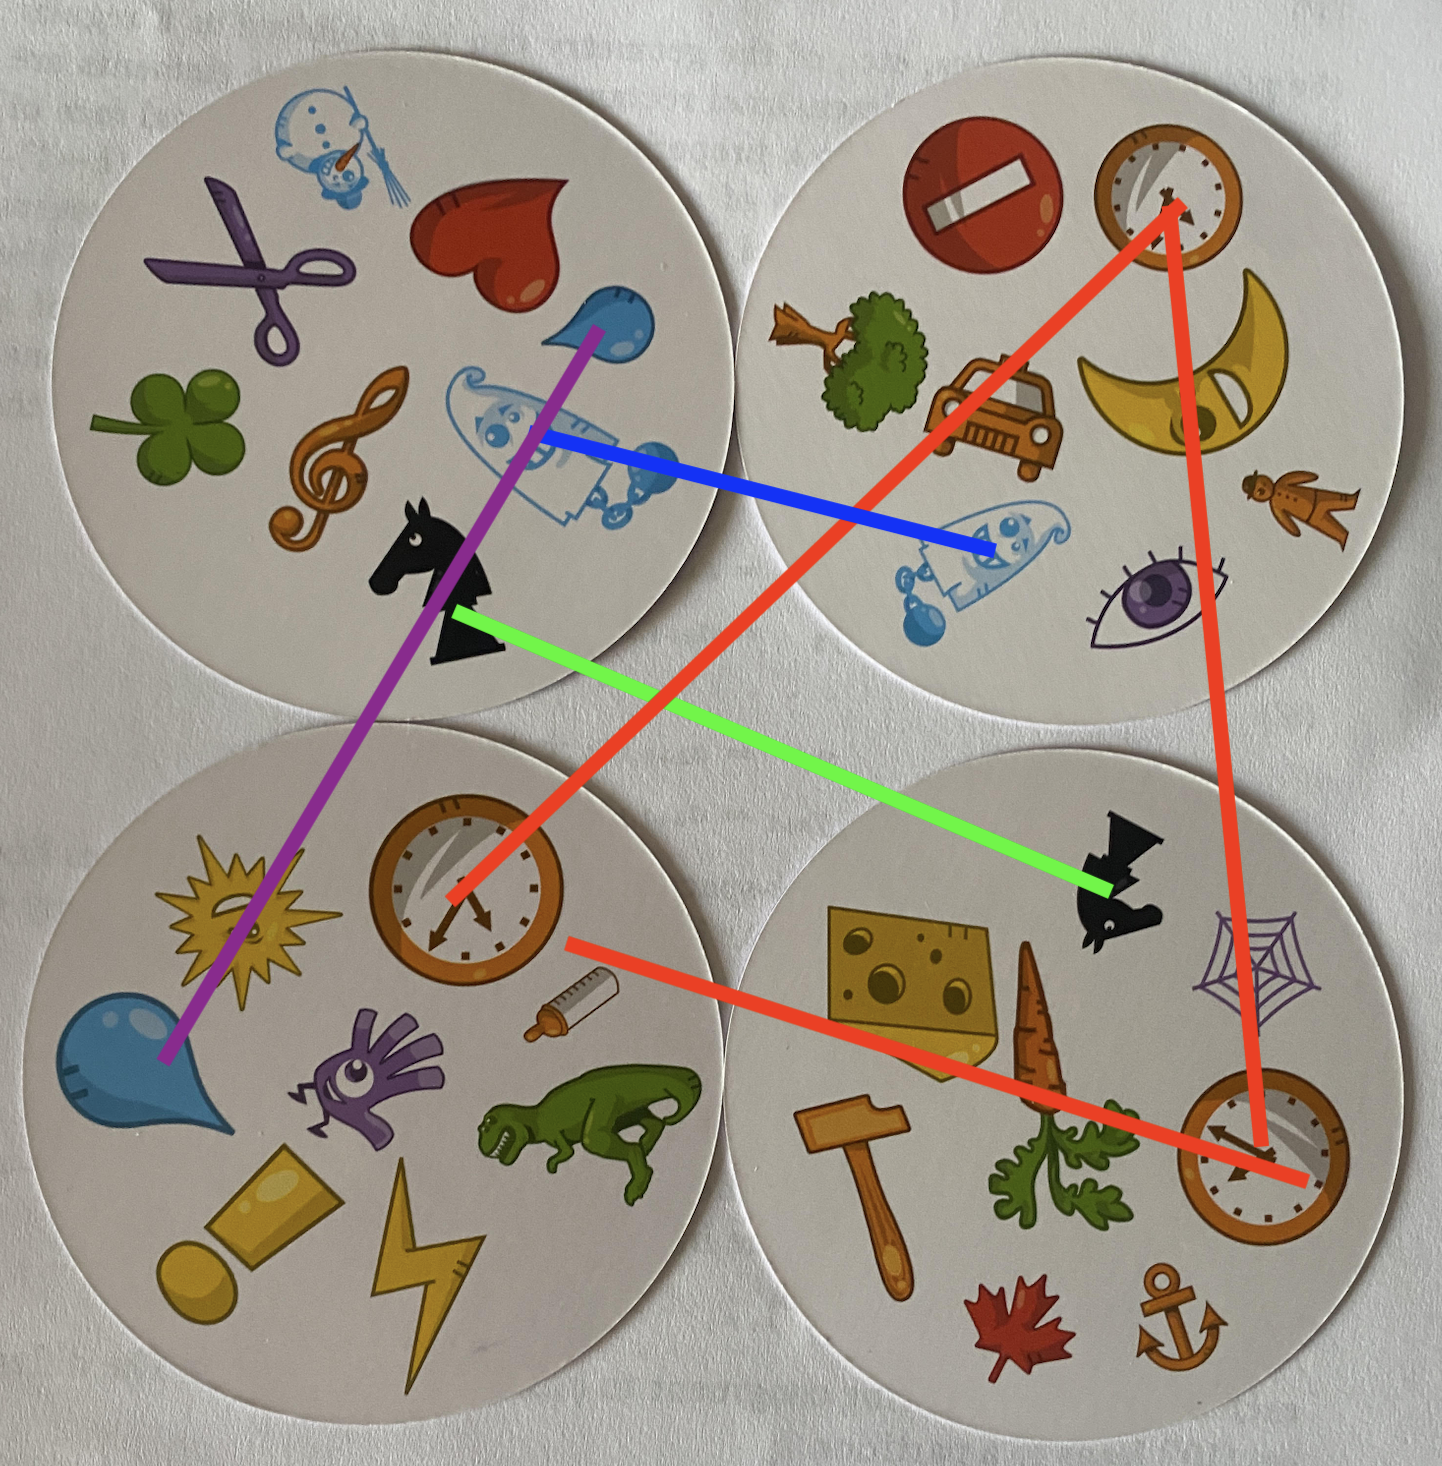
\includegraphics[scale=.2]{cards-links}
\caption{Four cards in the game with links}
\label{fig:cards-links}
\end{subfigure}

\begin{subfigure}{.2\textwidth}
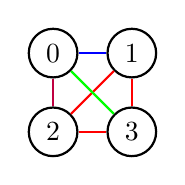
\begin{tikzpicture}
\begin{scope}[every node/.style={circle,thick,draw}]
\node (0) at (0, 1) {0}; 
\node (1) at (1, 1) {1}; 
\node (2) at (0, 0) {2}; 
\node (3) at (1, 0) {3}; 

\draw[thick, red] (1) -- (2); 
\draw[thick, red] (1) -- (3); 
\draw[thick, red] (2) -- (3); 

\draw[thick, blue] (0) -- (1); 
\draw[thick, green] (0) -- (3); 
\draw[thick, purple] (0) -- (2); 
\end{scope}
\end{tikzpicture}
\caption{Four cards graph, with cards as nodes and an edge color for each shared symbol}
\label{fig:cards-graph}
\end{subfigure}

\end{figure}

Naturally, there are trivial constructions: every symbol occurs only twice, or once, or the count of symbols is so varied that a deck can be constructed almost greedily. However, the Spot It game has uniformly 8 symbol ``slots'' on each card, which each appear 8 times\footnote{As we will see later, there should be 57 cards for this to be true; it's likely two cards were removed} across the different cards. 

This is what we examine in this paper:

\begin{framed}
\textbf{The Core Question:} For what choices of $g$ and $s$ can we construct a ``Spot It'' deck where each of the $s$ symbols on each card appears exactly $g$ times throughout the deck?
\end{framed}

\subsection{Reframing as a graph problem}
Noticing that every card has a relationship to every other card (notably, the identity of the single symbol shared between them) as in Fig.~\ref{fig:cards-links}, we take our first step by reconstructing this problem as an undirected graph as in Fig.~\ref{fig:cards-graph}. 


\begin{figure}[!htb]
\centering
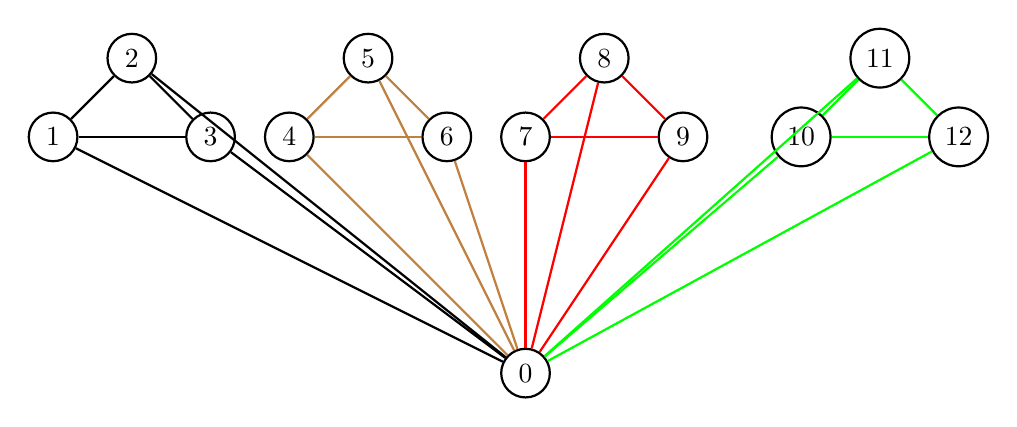
\begin{tikzpicture}
\begin{scope}[every node/.style={circle,thick,draw}]
\node (0) at (0, -2) {0}; 
\node (1) at (-6, 1) {1}; 
\node (2) at (-5, 2) {2}; 
\node (3) at (-4, 1) {3}; 
\node (4) at (-3, 1) {4}; 
\node (5) at (-2, 2) {5}; 
\node (6) at (-1, 1) {6}; 

\node (12) at (5.5, 1) {12}; 
\node (11) at (4.5, 2) {11}; 
\node (10) at (3.5, 1) {10}; 
\node (9) at (2, 1) {9}; 
\node (8) at (1, 2) {8}; 
\node (7) at (0, 1) {7}; 

\draw[thick, black] (0) -- (1); 
\draw[thick, black] (0) -- (2); 
\draw[thick, black] (0) -- (3); 

\draw[thick, black] (2) -- (3); 
\draw[thick, black] (1) -- (2); 
\draw[thick, black] (1) -- (3); 


\draw[thick, brown] (0) -- (4); 
\draw[thick, brown] (0) -- (5); 
\draw[thick, brown] (0) -- (6); 

\draw[thick, brown] (5) -- (6); 
\draw[thick, brown] (4) -- (5); 
\draw[thick, brown] (4) -- (6); 


\draw[thick, red] (0) -- (7); 
\draw[thick, red] (0) -- (8); 
\draw[thick, red] (0) -- (9); 


\draw[thick, red] (8) -- (9); 
\draw[thick, red] (7) -- (8); 
\draw[thick, red] (7) -- (9); 


\draw[thick, green] (0) -- (10); 
\draw[thick, green] (0) -- (11); 
\draw[thick, green] (0) -- (12); 


\draw[thick, green] (11) -- (12); 
\draw[thick, green] (10) -- (11); 
\draw[thick, green] (10) -- (12); 

\end{scope}
\end{tikzpicture}
\caption{$n = s(g-1)+1$. Here, $s=4, g=3$}
\label{fig:graph-theorem}
\end{figure}


\begin{framed}
\textbf{The Graph Representation:} A deck of Spot It Cards each with $s$ symbol slots, where each symbol appears $g$ times, can be represented by a graph $G$:
\begin{enumerate}
\item With $n$ nodes, where $n = s(g-1) + 1$,
\item With $m$ unique edge colors, where $m$ denotes the number of unique symbols, and
\item Where all edges each of color $m_i$ form a complete subgraph on $g$ nodes, so $m = {n \choose 2} / {g \choose 2}$.
\end{enumerate}
\end{framed}

\emph{Note: Singletons (groups where $g=1$) would be rendered as self-edges. These are uninteresting and are generally ignored in this paper}

\emph{Proof}:
\begin{enumerate}
\item As in Fig.~\ref{fig:graph-theorem}, node $n_0$'s adjacencies are exactly $s$ monocolor cliques of size $g-1$ (excluding $n_0$ itself). In a complete graph, these adjacencies comprise the total node set, so $n = (g-1)s + 1$. Using any other node is equivalent.
\item As in Fig.~\ref{fig:cards-links}, while card 1 and card 2 have the relationship ``clock'', node 1 and node 2 instead share an edge with the color red. This is the same relationship between nodes 2 and 3, and nodes 1 and 3. ``Drop'', ``knight'', and ``ghost'' would be colors purple, green, and blue, respectively. This works because every edge has exactly one color (corresponding 1:1 with a symbol) in this formulation, and every card pair shares exactly one symbol.
\item All cards with a given symbol (say, ``clock'') must link via a single color (here, red) to all other nodes whose card has that symbol; this is a complete subgraph. A complete graph $K_n$ has ${n \choose 2}$ edges. A monocolor clique of size $g$ is a complete graph as well, with ${g \choose 2}$ edges. $K_n$'s edges are exactly these equal-sized cliques, so there are therefore $m = \frac{{n \choose 2}}{{g \choose 2}}$ of them, corresponding to colors.
\end{enumerate}

And since every edge in our complete graph $K_n$ is in exactly one monocolor clique of size $K_g$, this becomes a crisp graph theory problem:

\begin{framed}
\textbf{The Core Question in Graph Terms}: Given $s$ and $g$ as before, can we construct an edge partition (colloquially here, ``coloring'') of a complete graph on $n$ nodes $K_n$ into a set of complete subgraphs of size $g$ (denoted $K_g$)?
\end{framed}

\emph{Note: Our idiosyncratic term ``coloring'', which really just serves to better visualize partitioning a graph into disjoint edge sets, should not be confused with the traditional term ``edge coloring'', where no edges of the same color can meet at a node. Also, we sometimes sloppily use ``clique'', ``group'', and ``complete subgraph'' interchangeably to mean ``the entire set of nodes connected by one color of edge''}.

\textbf{Though exhaustive research wasn't done, this graph problem does not appear to have a clear analytical solution out there.}\footnote{Or people who care about publishing it within the reach of lazy hobbyists, anyway!}

Since $m$ and $n$ are determined from $s$ and $g$, we'll start by looking at possible candidate configurations of $s$ and $g$.

\section{The Candidate Theorem: $g | s(s-1), g \leq s$}

Suppose that that every card has $s$ symbols, and any symbols hzx exactly $g$ cards containing it\footnote{for example, all cards contain $s=4$ symbols in Fig.~\ref{fig:s4g3}, which each appear on $g=3$ cards}. Then 

\begin{framed}
\begin{enumerate}
\item $g | s(s-1)$.
\item If $s >1 $ and $g > 1$ then $g \leq s$ 
\item If $s >1 $ and $g > 1$, then $m = (\frac{s}{g})n$ and therefore $m \geq n$
\item All nontrivial candidate configurations of $g, s$ are then $g \leq s$, $g | s(s-1)$.
\end{enumerate}
\end{framed}

\emph{Proof}:
\begin{enumerate}
\item 
\begin{align}
{g \choose 2} \bigg| {n \choose 2} \Rightarrow \frac{n(n-1)}{g(g-1)} \in \mathbb{N} \Rightarrow g(g-1) | n(n-1) \\
 n = (g-1)s+1 \Rightarrow g(g-1) \big| (sg-s+1)(sg-s) = (sg-s+1)s(g-1)\\
\Rightarrow g | s^2g - s^2 + s \Rightarrow g | (1-s)s \Rightarrow g | s(s-1) 
\end{align}
\item Any node $n_i$ is adjacent to $s$ monocolor cliques of size $g$. These cliques $C_1 ... C_s$ (containing non-$n_i$ nodes if $g > 1$) comprise all nodes, and any other cliques can contain no more than one of each $C_i$. This means that clique of size $g$ greater than $s$ cannot be formed, since the only place to find nodes are these $C_1 ... C_s$. The other trivial case, $s=1$, means there is only one color in the whole graph. 
\\

This means we need not consider configurations like $g = 6, s=3$ even though $6 | 3(3-1)$.

\item Another corollary here is that \fbox{$m \geq n$}, since:
\begin{align}
n = (sg - s + 1) \\
m = \frac{{(sg - s + 1)(sg-s) \choose 2}}{{g \choose 2}} = \frac{(sg-s+1)(sg-s)}{g(g-1)} = \frac{(sg-s+1)s}{g} \\
\Rightarrow m = (\frac{s}{g})n\\
s \geq g \Rightarrow m \geq n
\end{align}
\item This is just a combination of (1) and (2). But for example, a tiling of triangles ($g=3$) means that either $s \equiv 0 \mod 3$ (see Fig.~\ref{fig:s3g3})
 or $s \equiv 1 \mod 3$ (see Fig.~\ref{fig:s4g3}). 
\end{enumerate}




\begin{figure}[!htb]
\centering
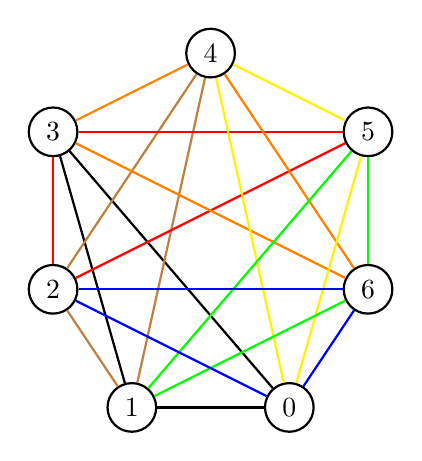
\begin{tikzpicture}
\begin{scope}[every node/.style={circle,thick,draw}]
 \node (0) at (3,0.5) {0};
 \node (1) at (1,0.5) {1};
 \node (2) at (0,2) {2};
 \node (3) at (0,4) {3};
 \node (4) at (2,5) {4};
 \node (5) at (4,4) {5};
 \node (6) at (4,2) {6};
 
 
\draw[thick, black] (0) -- (1); 
\draw[thick, black] (1) -- (3); 
\draw[thick, black] (0) -- (3); 

\draw[thick, brown] (1) -- (2); 
\draw[thick, brown] (2) -- (4); 
\draw[thick, brown] (1) -- (4); 

\draw[thick, red] (2) -- (3); 
\draw[thick, red] (3) -- (5); 
\draw[thick, red] (2) -- (5); 

\draw[thick, orange] (3) -- (4); 
\draw[thick, orange] (4) -- (6); 
\draw[thick, orange] (3) -- (6); 

\draw[thick, yellow] (4) -- (5); 
\draw[thick, yellow] (5) -- (0); 
\draw[thick, yellow] (4) -- (0); 

\draw[thick, green] (5) -- (6); 
\draw[thick, green] (6) -- (1); 
\draw[thick, green] (5) -- (1); 

\draw[thick, blue] (6) -- (0); 
\draw[thick, blue] (0) -- (2); 
\draw[thick, blue] (6) -- (2); 


\end{scope}
\end{tikzpicture}
\caption{s=3, g=3, n=7, m=7. Cliques of form $(n_i, n_{i+1}, n_{i+3}), \forall i$}
\label{fig:s3g3}
\end{figure}




\begin{figure}[!htb]
\centering
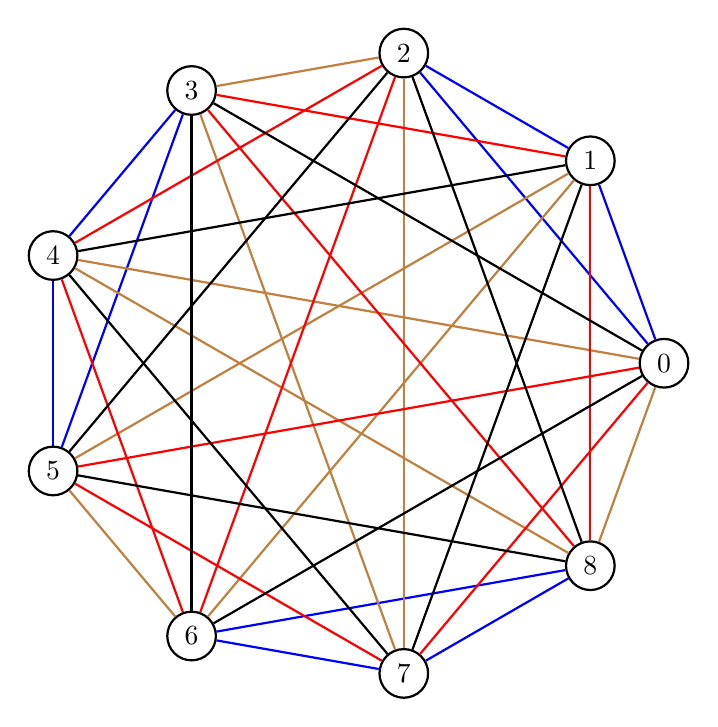
\begin{tikzpicture}
\begin{scope}[every node/.style={circle,thick,draw}]

\node (0) at (4,0) {0};
\node (1) at (3.064,2.571) {1};
\node (2) at (0.695,3.939) {2};
\node (3) at (-2,3.464) {3};
\node (4) at (-3.759,1.368) {4};
\node (5) at (-3.759,-1.368) {5};
\node (6) at (-2,-3.464) {6};
\node (7) at (0.695,-3.939) {7};
\node (8) at (3.064,-2.571) {8};
 
\draw[thick, blue] (0) -- (1); 
\draw[thick, blue] (1) -- (2); 
\draw[thick, blue] (0) -- (2); 

\draw[thick, blue] (3) -- (4); 
\draw[thick, blue] (4) -- (5); 
\draw[thick, blue] (3) -- (5); 

\draw[thick, blue] (6) -- (7); 
\draw[thick, blue] (7) -- (8); 
\draw[thick, blue] (6) -- (8); 

\draw[thick, brown] (0) -- (4); 
\draw[thick, brown] (0) -- (8); 
\draw[thick, brown] (4) -- (8); 

\draw[thick, brown] (3) -- (7); 
\draw[thick, brown] (3) -- (2); 
\draw[thick, brown] (7) -- (2); 

\draw[thick, brown] (6) -- (1); 
\draw[thick, brown] (6) -- (5); 
\draw[thick, brown] (1) -- (5); 

\draw[thick, red] (0) -- (5); 
\draw[thick, red] (0) -- (7); 
\draw[thick, red] (5) -- (7); 

\draw[thick, red] (3) -- (8); 
\draw[thick, red] (3) -- (1); 
\draw[thick, red] (8) -- (1); 

\draw[thick, red] (6) -- (2); 
\draw[thick, red] (6) -- (4); 
\draw[thick, red] (2) -- (4); 


\draw[thick, black] (0) -- (3); 
\draw[thick, black] (0) -- (6); 
\draw[thick, black] (3) -- (6); 

\draw[thick, black] (1) -- (4); 
\draw[thick, black] (1) -- (7); 
\draw[thick, black] (4) -- (7); 

\draw[thick, black] (2) -- (5); 
\draw[thick, black] (2) -- (8); 
\draw[thick, black] (5) -- (8); 


\end{scope}



\end{tikzpicture}
\caption{s=4, g=3, n=9, m=12. \\
Cliques: $(n_i, n_{i+3}, n_{i+6}), (n_i, n_{i+1}, n_{i+2}), (n_i, n_{i+4}, n_{i+8}) \forall i, (n_i, n_{i+5}, n_{i+7}), i \equiv 0 \mod 5 $}
\label{fig:s4g3}
\end{figure}



\section{Constructing $g = s-1$ over a field}

Though we presented a few legitimate examples of complete graphs tiled by uniformly sized complete subgraphs in Fig.~\ref{fig:s3g3} and Fig.~\ref{fig:s4g3}, these are not easy to find by hand once $s$ becomes much larger. The whole problem of graph partitioning admits many algorithms, most approximations\cite{3}, though usually referring to separating actual \emph{nodes} into partitions, rather than edges, and usually over an arbitrary graph instead of a relatively simple complete graph.

We can, however, systematically construct an edge partition if $g$ is a prime power.

\begin{framed}
\textbf{g=s-1 construction}: If $g$ is a prime power $p^k$, we can explicitly construct a graph that satisfies our game with $g = s-1$.
\end{framed}


As the combination of $s, g$ determine the shape of the graph entirely, $g = s-1$ implies:
\begin{itemize}
\item The graph has $n = s(g-1) + 1 = (g+1)(g-1) + 1 = g^2$ nodes.
\item Those nodes can be grouped into $g$ groups of size $g$.
\item There are $m = (\frac{s}{g}) n = (\frac{s}{g}) g ^2 = sg = (g+1)g$ colors in the graph.
\end{itemize}

\subsection{General Construction Algorithm}
\emph{Algorithm Summary}: Our algorithm takes every constant $c \in \mathcal{F}$, and goes through the multiplication table of $\mathcal{F}$ row ($y$) by row.  To a clique $C_{c,y}$ specified by these two,  we add an element from $G_x$ for every column $x$ : The entry from $G_x$ indexed by the entry at $z = (x,y)$ in the table, plus the constant $c$.

\begin{framed}
\textbf{Construction Algorithm for $g=s-1$:}

To construct the $m = g(g-1)$ colors (symbol cliques) in the graph:
\begin{itemize}
 \item Construct a finite field $\mathcal{F} = \mathcal{GF}(g) $, which is of size $g$.
 \item Divide the $g^2$ nodes into $g$ cliques $(G_0, G_1, ... G_{g-1})$, where $[0...g-1] \in \mathcal{F}$, of $g$ nodes each $(G_{0,0}, G_{0,1}...G_{0,g-1}) ...(G_{g-1,0}, G_{g-1,1}...G_{g-1,g-1})$
 \item For all $c \in [0,g-1]$: 
 \begin{itemize}
 \item For all $y \in [0,g-1]$: 
 \begin{itemize}
 \item Create clique $C_{c,y}$, initially the empty set.  $y$ is the row (specifying the multiplier) and $c$ is a constant (added to each result).
 \item For all $x \in [0,g-1]$, set $z = G_x \cdot G_y + c$, where $+$ and $\cdot$ refer to addition and multiplication rules for $\mathcal{F}$, and add $G_{x, z}$ to clique $C_{c, y}$.
 \end{itemize}
 \end{itemize}
 \item The cliques $(G_0, G_1, ... G_{g-1})$, plus the $g^2$ cliques like $C_{c, y}$ form the $(g+1)g$ cliques or ``colors''.
\end{itemize}
\end{framed}


\subsection{Constructing with prime $g$}

We can start with the easiest way to see this: $g = p, p \in \mathbb{P}$.

Let's construct the operation tables for the finite field on $p=3$, as in Fig.~\ref{fig:gf3-tables}.



\begin{figure}[!htb]
\centering
\begin{subfigure}{.3\textwidth}
 \centering
 \begin{tabular}{c | c c c}
 + & 0 & 1 & 2 \\
\hline
 0 & 0 & 1 & 2 \\
 1 & 1 & 2 & 0 \\
 2 & 2 & 1 & 0 \\
 \end{tabular}
 \caption{Addition table GF(3)}
\label{fig:gf3-add}
\end{subfigure}
\begin{subfigure}{.3\textwidth}
 \centering
\begin{tabular}{c | c c c}
 $\cdot$ & 0 & 1 & 2 \\
\hline
 0 & 0 & 0 & 0 \\
 1 & 0 & 1 & 2 \\
 2 & 0 & 2 & 1 \\

\end{tabular}
\caption{Multiplication table GF(3)}
\label{fig:gf3-mult}
\end{subfigure}
\caption{Field tables for GF(3)}
\label{fig:gf3-tables}
\end{figure}



\begin{figure}[!htb]
\centering
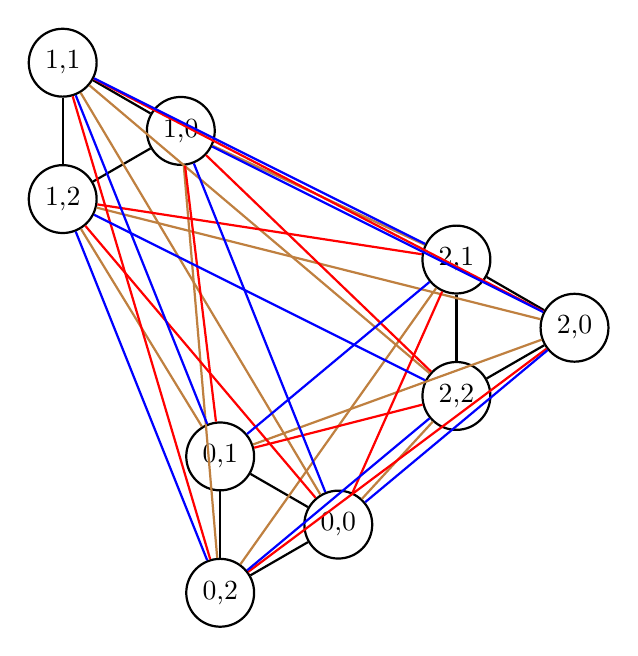
\begin{tikzpicture}
\begin{scope}[every node/.style={circle,thick,draw}]
\node (0) at (1,0) {0,0}; 
\node (1) at (-.5, .866) {0,1}; 
\node (2) at (-.5, -.866) {0,2}; 

\node (3) at (-1,5) {1,0}; 
\node (4) at (-2.5, 5.866) {1,1}; 
\node (5) at (-2.5, 4.134) {1,2}; 

\node (6) at (4,2.5) {2,0}; 
\node (7) at (2.5, 3.366) {2,1}; 
\node (8) at (2.5, 1.634) {2,2}; 


\draw[thick, black] (0) -- (1); 
\draw[thick, black] (1) -- (2); 
\draw[thick, black] (0) -- (2); 

\draw[thick, black] (3) -- (4); 
\draw[thick, black] (4) -- (5); 
\draw[thick, black] (3) -- (5); 

\draw[thick, black] (6) -- (7); 
\draw[thick, black] (7) -- (8); 
\draw[thick, black] (6) -- (8); 

\draw[thick, brown] (0) -- (4); 
\draw[thick, brown] (0) -- (8); 
\draw[thick, brown] (4) -- (8); 

\draw[thick, brown] (3) -- (7); 
\draw[thick, brown] (3) -- (2); 
\draw[thick, brown] (7) -- (2); 

\draw[thick, brown] (6) -- (1); 
\draw[thick, brown] (6) -- (5); 
\draw[thick, brown] (1) -- (5); 

\draw[thick, red] (0) -- (5); 
\draw[thick, red] (0) -- (7); 
\draw[thick, red] (5) -- (7); 

\draw[thick, red] (3) -- (8); 
\draw[thick, red] (3) -- (1); 
\draw[thick, red] (8) -- (1); 

\draw[thick, red] (6) -- (2); 
\draw[thick, red] (6) -- (4); 
\draw[thick, red] (2) -- (4); 


\draw[thick, blue] (0) -- (3); 
\draw[thick, blue] (0) -- (6); 
\draw[thick, blue] (3) -- (6); 

\draw[thick, blue] (1) -- (4); 
\draw[thick, blue] (1) -- (7); 
\draw[thick, blue] (4) -- (7); 

\draw[thick, blue] (2) -- (5); 
\draw[thick, blue] (2) -- (8); 
\draw[thick, blue] (5) -- (8); 

\end{scope}

\end{tikzpicture}
\caption{whole $K_9$: $s=4, g=3, n=9, m=12$}
\label{fig:k9}

\end{figure}

Refer to Fig.~\ref{fig:k9}.

\begin{enumerate}
\item Cliques $G_0, G_1, G_2$: these are the triangles in black. 
\item Cliques $C_{0,0}, C_{1, 0}, C_{2,0}$: these are the triangles in blue. These walk through the $0$ row in the multiplication table in Fig.~\ref{fig:gf3-mult}.
\item Cliques $C_{0,1}, C_{1, 1}, C_{2,1}$: these are the triangles in brown.  These walk through the $1$ row in the multiplication table in Fig.~\ref{fig:gf3-mult}.
\item Cliques $C_{0,1}, C_{1, 1}, C_{2,1}$: these are the triangles in red. These walk through the $2$ row in the multiplication table in Fig.~\ref{fig:gf3-mult}.
\end{enumerate}


Every node is connected to every other node once in Fig.~\ref{fig:k9}, since for nodes $x,y$ and $z,w$:
\begin{itemize}
\item If $x = z$, they're in the same ``black'' clique $G_x$.
\item If $y=w$, they're in a ``blue'' clique $C_{c,0}$, where our multiplier $y$ is zero.  Every member of $C_{2,0}$, for example, is the 2 element of their $G_i$: $G_{0,2}, G_{1,2}, G_{2,2}$.
\item Else there is some multiplier $a$ where starting from node ($x,y)$, going $z-x$ mutlipicative ``hops'' away lands us at node $w$.  These are like the brown ($a=1$) or red ($a=2\equiv -1 \mod 3 $) cliques.
\end{itemize}

Compare identical graphs Fig.~\ref{fig:k9} (generated from the algorithm) and Fig.~\ref{fig:s4g3}. The mapping between node $(i,j)$ in Fig.~\ref{fig:k9} and node $k$ in Fig.~\ref{fig:s4g3} is $(i,j) \rightarrow k=i+3j$, with inverse $k \rightarrow (k \mod 3, \lfloor k / 3 \rfloor)$.  In Fig.~\ref{fig:s4g3}:
\begin{itemize}
\item The black cliques are $\{G_0, G_3, G_6\}, \{G_1, G_4, G_7\}, \{G_2, G_5, G_8\}$, grouped by $i \mod n$.
\item The blue cliques are $\{G_0, G_1, G_2\}, \{G_3, G_4, G_5\}, \{G_6, G_7, G_8\}$, a walk through the top row of Fig.\ref{fig:gf3-mult}.
\item The brown cliques are $\{G_0, G_4, G_8\}, \{G_6, G_1, G_5\}, \{G_3, G_7, G_8\}$, a walk through the second row of Fig.\ref{fig:gf3-mult}.
\item The red cliques are $\{G_0, G_7, G_5\}, \{G_3, G_1, G_8\}, \{G_6, G_4, G_2\}$, a walk through the third row of Fig.\ref{fig:gf3-mult}.
\end{itemize}

\subsection{Constructing for g as prime power}

For prime numbers, it's clear that every increment in $[1, p-1]$ traverses a path $a, 2a, 3a ... (p-1)a$ where the nth member is unique among all other increment paths.

The leap of insight comes in realizing that, in general, these cliques are not additive increments, but journeys through a field's \emph{multiplication table}; for $g$ prime, these look additive, but for more complicated finite fields, we need to defer to the table.

We can do this for prime-power fields like $GF(2^2=4)$: 

\begin{figure}[!htb]
\centering
\begin{subfigure}{.3\textwidth}
 \centering
 \begin{tabular}{c | c c c c}
 + & 0 & 1 & B & D \\
\hline
 0 & 0 & 1 & B & D \\
 1 & 1 & 0 & D & B \\
 B & B & D & 0 & 1 \\
 D & D & B & 1 & 0 \\
 \end{tabular}
 \caption{Addition table GF(4)}
\label{fig:gf4-add}
\end{subfigure}
\begin{subfigure}{.3\textwidth}
 \centering
\begin{tabular}{c | c c c c}
 $\cdot$ & 0 & 1 & B & D \\
\hline
 0 & 0 & 0 & 0 & 0 \\
 1 & 0 & 1 & B & D \\
 B & 0 & B & D & 1 \\
 D & 0 & D & 1 & B \\
\end{tabular}
 \caption{Multiplication table GF(4)}
\label{fig:gf4-mult}
\end{subfigure}
\end{figure}

Unlike a prime-order finite field, the addition table is not cyclic, so in a sense, our indices for $G_{0,i}$ say are not $i \in [0, 3]$ but $i \in \{0,1,B,D\}$! This is why the phrase ``where $[0...g-1] \in \mathcal{F}$'' is important in the algorithm.

\begin{figure}[!htb]
\begin{subfigure}{.25\textwidth}
\begin{tabular}{|| c c || c c c c || } 
 \hline
c & y & $G_0$ & $G_1$ & $G_B$ & $G_D$ \\ [0.5ex] 
 \hline\hline
 0 & 0 & 0 & 0 & 0 & 0 \\
 0 & 1 & 0 & 1 & B & D \\
 0 & B & 0 & B & D & 1 \\
 0 & D & 0 & D & 1 & B \\
 \hline
 \end{tabular}
\caption{Cliques $C_{0,i}$}
\label{fig:cliques4-0}
\end{subfigure}
\begin{subfigure}{.25\textwidth}
\begin{tabular}{|| c c || c c c c || } 
 \hline
c & y & $G_0$ & $G_1$ & $G_B$ & $G_D$ \\ [0.5ex] 
 \hline\hline
 1 & 0 & 1 & 1 & 1 & 1 \\
 1 & 1 & 1 & 0 & D & B \\
 1 & B & 1 & D & B & 0 \\
 1 & D & 0 & B & 0 & D \\
 \hline
 
 \end{tabular}
\caption{Cliques $C_{1,i}$}
\label{fig:cliques4-1}
\end{subfigure}
\begin{subfigure}{.25\textwidth}
\begin{tabular}{|| c c || c c c c || } 
 \hline
c & y & $G_0$ & $G_1$ & $G_B$ & $G_D$ \\ [0.5ex] 
 \hline\hline
 \cellcolor{yellow}B & \cellcolor{yellow}0 & \cellcolor{yellow}B & \cellcolor{yellow}D & \cellcolor{yellow}0 & \cellcolor{yellow}1 \\
 \cellcolor{cyan}B & \cellcolor{cyan}1 & \cellcolor{cyan} B & \cellcolor{cyan}0 & \cellcolor{cyan}1 & \cellcolor{cyan} D \\
 B & B & B & 1 & D & 0 \\
 B & D & B & B & B & B \\
 \hline
 
 \end{tabular}
\caption{Cliques $C_{B,i}$}
\label{fig:cliques4-B}
\end{subfigure}
\begin{subfigure}{.25\textwidth}
\begin{tabular}{|| c c || c c c c || } 
 \hline
c & y & $G_0$ & $G_1$ & $G_B$ & $G_D$ \\ [0.5ex] 
 \hline\hline
 D & 0 & D & D & D & D \\
 D & 1 & D & B & 1 & 0 \\
 D & B & D & 1 & 0 & B \\
 D & D & D & 0 & B & 1 \\
 \hline
 
 \end{tabular}
\caption{Cliques $C_{D,i}$}
\label{fig:cliques4-D}
\end{subfigure}
\caption{s=5, g=4 adjacency tables}
\end{figure}

Here are the resulting tables for $s=5, g=4$. For example, in Fig.~\ref{fig:cliques4-0}, consider the third row as saying ``clique $C_{0,B}$ contains nodes $G_{0,0}, G_{1,B}, G_{B,D}, G_{D,1}$''.


(Of course, once the multiplication is defined, feel free to substitute 2 for $B$ and 3 for $D$, in, say, a program.)


Including the ``black'' cliques like $G_B = \{G_{0,B}, G_{1,B}, G_{2,B}, G_{3,B}\}$, we see that there are no repeated edges, and all edges are accounted for. 

In general, to prove that this table exactly represents the ``color'' of every edge, we need to show that for every pair of elements, say, $(B, 1)$, and every pair of columns, say $0$ and $B$, (see the blue row in Fig.~\ref{fig:cliques4-B}) that B and 1 appear in the same row in columns 0 and B exactly once. 

\emph{Proof}:
To ensure there are no duplicates, consider two columns $x_1$ and $x_2$ that have a repeated value pair in some table, once on the table row beginning $(c, g_y)$, once on $(c^*, g_y^*)$:

\begin{itemize}
\item Assume $g_yg_{x_1} + c = g_y^*g_{x_1} +c^*$, and $g_yg_{x_2} + c = g_y^*g_{x_2} +c^*$ for $g_{x_1} \neq g_{x_2}$
\item Subtract the two to get $g_y(g_{x_1} - g_{x_2}) = g_y^*(g_{x_1} - g_{x_2})$
\item The field $\mathcal{F}$ requires the nonzero $(g_{x_1} - g_{x_2}) \in \mathcal{F}$ to have an inverse. 
\item Multiplying both sides by that inverse, we have $g_y = g_y^*$, showing they cannot be distinct. Thus, we have no duplicates.
\end{itemize}

Similar field-based arguments can be made to ensure that every pair is represented. Since everything we're dealing with is finite, however, we can also use a pigeonhole approach:
\begin{itemize}
\item For any pair of columns, there are $g^2$ pairs of values to account for.
\item Across the tables above, there are $g^2$ rows (combinations of $c$ and $y$ that generate the cliques).
\item From the previous arugment, no two rows can be duplicated.
\item Therefore, by the pigeonhole principle, every combination is represented, and therefore, between any two $G_j$ cliques, every node has an edge with every other.
\end{itemize}


\section{Constructing $g=s$ from $g=s-1$}

With the previous construction ($g=s-1$) in hand, we can easily construct a $g=s$ graph (adding one to $g$, keeping $s$ the same), with the same restrictions on $g$. See Fig.~\ref{fig:s5g5} for a visual on this.

\begin{itemize}
\item Create node $n_y$ for $y \in \mathcal{F}$
\item Add $n_y$ to all cliques $C_{c, y}$. For a given $y$, these cliques share no nodes.
\item Create node $n^*$. Add this to every $G_i$ clique.
\item Create clique of all $n_y, y \in [0, g]$ plus $n^*$.
\end{itemize}

We see then that:

\begin{itemize}
\item Every new node $n_y$ gets added to the new ``n'' clique plus $s-1$ cliques, all of size $s$.
\item $n^*$ is added to $s-1$ cliques plus the bottom clique.
\item Every $G$-style clique gets $n^*$ added to it.
\item Every $C_{c,y}$ clique adds node $n_y$.
\item So, the new partition is one where $g=s$, built on the previous where $g=s-1$.
\end{itemize}

\emph{Note that you can create $s=g=8$ this way, with $n=m=57$. The Spot It card deck comes with 55 cards with $s=8$ ``slots'', so our suspicion is that two cards were simply dropped from the set},.



\begin{figure}[!htb]
\centering
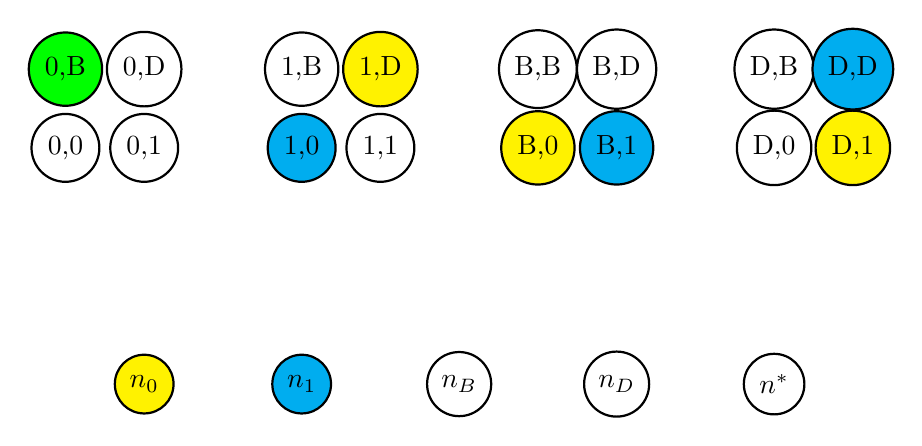
\begin{tikzpicture}
\begin{scope}[every node/.style={circle,thick,draw}]
\node (0)at (0,0) {0,0}; 
\node (1) at (1,0) {0,1}; 
\node (2) [fill=green] at (0,1) {0,B}; 
\node (3) at (1,1) {0,D}; 


\node (4)[fill=cyan] at (3,0) {1,0}; 
\node (5) at (4,0) {1,1}; 
\node (6) at (3,1) {1,B}; 
\node (7)[fill=yellow] at (4,1) {1,D}; 

\node (8)[fill=yellow] at (6,0) {B,0}; 
\node (9)[fill=cyan] at (7,0) {B,1}; 
\node (10) at (6,1) {B,B}; 
\node (11)at (7,1) {B,D}; 



\node (12) at (9,0) {D,0}; 
\node (13)[fill=yellow] at (10,0) {D,1}; 
\node (14) at (9,1) {D,B}; 
\node (15)[fill=cyan] at (10,1) {D,D}; 


\node (16)[fill=yellow] at (1,-3) {$n_0$}; 
\node (17)[fill=cyan] at (3,-3) {$n_1$}; 
\node (18) at (5,-3) {$n_B$}; 
\node (19) at (7,-3) {$n_D$}; 
\node (20) at (9, -3) {$n^*$}; 


\end{scope}
\end{tikzpicture}
\caption{s=5, g=5 created from s=5, g=4, no edges shown. The blue is the $C_{B,1}$ clique newly adding in $n_1$. The yellow is the $C_{0,1}$ clique newly adding in $n_0$. Node $0,B$ is in both.}
\label{fig:s5g5}
\end{figure}



\section{Alternative: Constructing $g=s$ with perfect difference sets}
\emph{Though it will be shown equivalent to the last construction, we can use another concept to build these graphs when $g=s$: perfect difference sets. Notably, these are proven to exist for $g=p^k-1$ by Singer\cite{1}}.

Searching for complete graph partitions by brute force is difficult. Even a graph of size 7 like Fig.~\ref{fig:s3g3} requires sorting through putting 21 distinct objects into 7 distinct bins\footnote{$(21!)/((3!)^7)$, though with some symmetries}, and the numbers get worse from there. 

There is some hope that a partition or coloring, should it exist, would exhibit some regularity; after all, every node has an equal configuration of edges and adjacent nodes in a complete graph.

Additionally, when $g=s$, we've seen that $n = m$, so finding a unique complete subgraph $K_g$ mapped 1:1 to each node which, in total, partition the complete graph, seems like a good strategy.

Looking at Fig.~\ref{fig:s3g3}, we see that every node at index $i$ can be mapped to a $K_3$ (color) whose vertices are $i$, $i+1$, and $i+3$, with addition being modulo 7. (Take a look at node 0's black triangle $(0, 1, 3)$. Beyond this, node $i$ needs to find adjacencies with node $i+2$, $i+4$, $i+5$, and $i+6$, or remapped over modulo 7, $i+2$, $i-3$, $i-2$, and $i-1$. However, we can find these latter four by simply repeating this triangle $(j, j+1, j+3)$ over the rest of the graph; in particular, the triangles at (i-1, i, i+2) (here, blue if $i=0$) and $(i-3, i-2, i)$ (yellow) take care of $i$'s six adjancies.

This works because among the $n=7$ nodes in this graph $g=s=3$, we found a complete graph $K_3$(in this case among nodes $\{0, 1, 3\}$) such that every chord length in $[1, \frac{n-1}{2}]\mod n$ is represented exactly once. Thinking of creating adjacencies for node 0, this means that connections to $\{1, 3\}$ will be taken care of by the associated triangle, that a $2$-chord exists by virtue of the triangle, and that $\{-1, -2, -3\}$ will be symmetrically connected \emph{to} 0 by the same means.

So, if for a given $n$, we can find a set $a_i \in [1,n-1]$ of size $g-1$ such that $\bigcup_{i > j} (a_i - a_j \mod n) = [1, \frac{n-1}{2}]$, then this can be repeated for every node to cover the graph.

That such a set exists is not obvious. However, through some basic search algorithms at \url{https://github.com/fettermania/mathnotes/tree/main/spotit/code}, we can sniff out a few of them:

\begin{figure}[!htb]
 \begin{tabular}{c c | c }
 g,s & n & 0 adjacencies \\
\hline
 3 & 7 & \{1, 3\} \\
 4 & 13 & \{1, 3, 9\} \\
 5 & 21 & \{1,4,14,16\} \\
 6 & 31 & \{1, 3, 8, 12, 18\} \\
 8 & 57 & \{1, 3, 13, 32, 36, 43, 52\} \\
 9 & 73 & \{1, 3, 7, 15, 31, 36, 54, 63\} \\
 10 & 91 & \{1, 3, 9, 27, 49, 56, 61, 77, 81\} \\
 12 & 133 & \{1, 3, 12, 20, 34, 38, 81, 88, 94, 104, 109\} \\
 \end{tabular}
 \caption{Perfect Difference Sets up to $g=s=12$}
\label{fig:perfect-diffs}
\end{figure}

Fig.~\ref{fig:s6g6} is an example of 0's adjacencies for $s=g=6$: 

\begin{figure}[!htb]
\centering
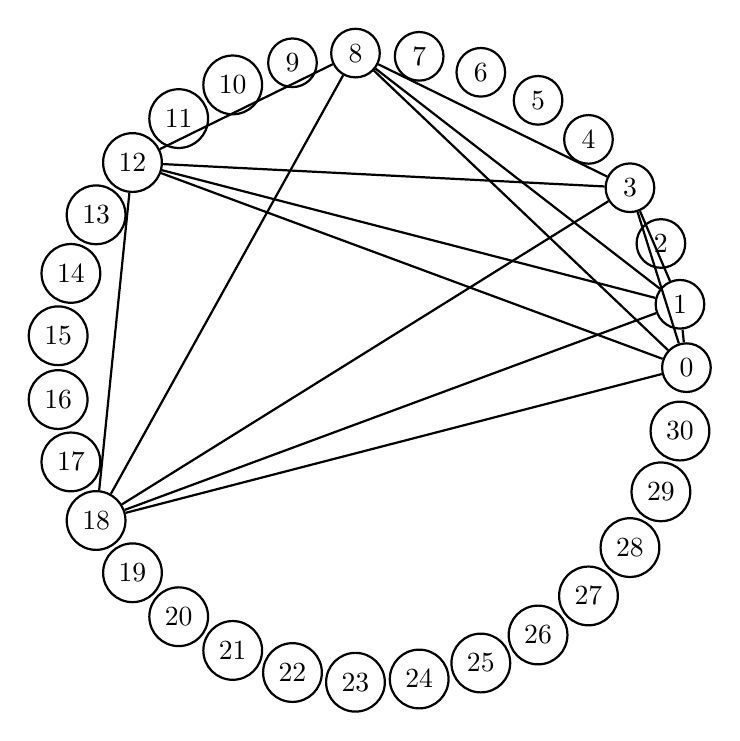
\begin{tikzpicture}
\begin{scope}[every node/.style={circle,thick,draw}]
\node (0) at (4,0) {0};
\node (1) at (3.918,0.805) {1};
\node (2) at (3.676,1.577) {2};
\node (3) at (3.283,2.285) {3};
\node (4) at (2.756,2.899) {4};
\node (5) at (2.116,3.395) {5};
\node (6) at (1.389,3.751) {6};
\node (7) at (0.606,3.954) {7};
\node (8) at (-0.203,3.995) {8};
\node (9) at (-1.003,3.872) {9};
\node (10) at (-1.762,3.591) {10};
\node (11) at (-2.448,3.163) {11};
\node (12) at (-3.035,2.605) {12};
\node (13) at (-3.497,1.941) {13};
\node (14) at (-3.817,1.197) {14};
\node (15) at (-3.979,0.405) {15};
\node (16) at (-3.979,-0.405) {16};
\node (17) at (-3.817,-1.197) {17};
\node (18) at (-3.497,-1.941) {18};
\node (19) at (-3.035,-2.605) {19};
\node (20) at (-2.448,-3.163) {20};
\node (21) at (-1.762,-3.591) {21};
\node (22) at (-1.003,-3.872) {22};
\node (23) at (-0.203,-3.995) {23};
\node (24) at (0.606,-3.954) {24};
\node (25) at (1.389,-3.751) {25};
\node (26) at (2.116,-3.395) {26};
\node (27) at (2.756,-2.899) {27};
\node (28) at (3.283,-2.285) {28};
\node (29) at (3.676,-1.577) {29};
\node (30) at (3.918,-0.805) {30};
 
 
 
\draw[thick, black] (0) -- (1); 
\draw[thick, black] (0) -- (3); 
\draw[thick, black] (0) -- (8); 
\draw[thick, black] (0) -- (12); 
\draw[thick, black] (0) -- (18); 

\draw[thick, black] (1) -- (3); 
\draw[thick, black] (1) -- (8); 
\draw[thick, black] (1) -- (12); 
\draw[thick, black] (1) -- (18); 

\draw[thick, black] (3) -- (8); 
\draw[thick, black] (3) -- (12); 
\draw[thick, black] (3) -- (18); 

\draw[thick, black] (8) -- (12); 
\draw[thick, black] (8) -- (18); 

\draw[thick, black] (12) -- (18); 


\end{scope}
,
\end{tikzpicture}
\caption{perfect difference set on g=6, s=6, n=m=31}
\label{fig:s6g6}
\end{figure}


It turns out that in the 1930s, James Singer found that these configurations, termed \emph{perfect difference sets}, exist for $g=p^k, p \in \mathbb{P}, k \in \mathbb{N}$ and, setting $n=g^2+g+1$\cite{1}. This result was not connected to graph edge partitioning in his paper. The existence for some of the other types of $g$ have been disproven, but this appears to be the main theorem in the area.


\begin{framed}
\textbf{Singer's Theorem on Perfect Difference Sets}: If $g=s$, then $n=g^2-g+1$ by the Graph Representation Theorem and $n=m$ by the Candidate Theorem. Thus, we're looking for a PDS over $n=g^2-g+1$. This has been proven to exist if $g =p^k, p \in \mathbb{P}, k \in \mathbb{N}$. 
\end{framed}

Singer's proof relies also on finding a finite field $\mathcal{F}$ of size g. There are some deterministic, non-brute-force methods of doing this\cite{4}, though they seem quite intricate.

This limitation to prime powers, just like the partitions for $g=s$ found in section 3, explains the row omissions in the brute force search table in Fig.~\ref{fig:perfect-diffs}. So, if $g=p^k+1$ a perfect difference set representation exists , and a section 3 representation also exists. 

\section{Interlude: Graph Equivalence up to relabeling}


\begin{figure}[!htb]
\centering
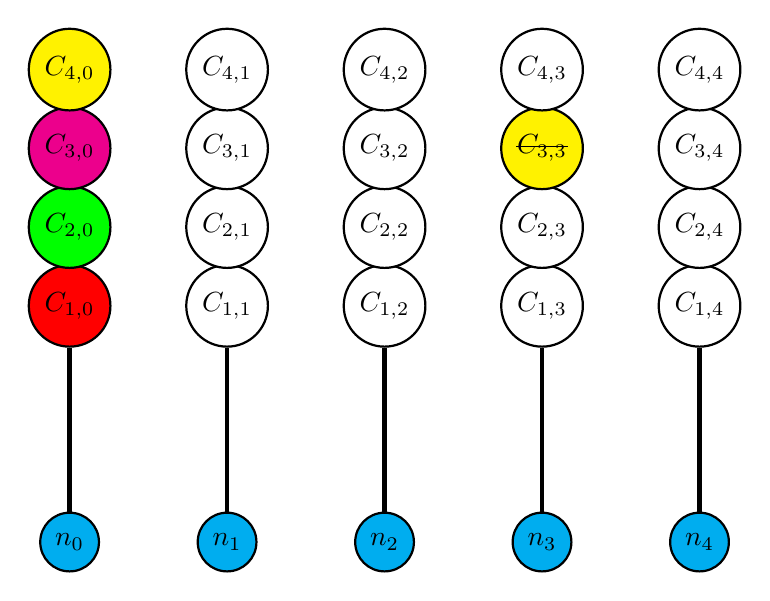
\begin{tikzpicture}
\begin{scope}[every node/.style={circle,thick,draw}]
\node (0)[fill=red] at (0,0) {$C_{1,0}$}; 
\node (1)[fill=green] at (0,1) {$C_{2,0}$}; 
\node (2)[fill=magenta] at (0,2) {$C_{3,0}$}; 
\node (3)[fill=yellow] at (0,3) {$C_{4,0}$}; 


\node (4)[fill=white] at (2,0) {$C_{1,1}$}; 
\node (5)[fill=white] at (2,1) {$C_{2,1}$}; 
\node (6)[fill=white] at (2,2) {$C_{3,1}$}; 
\node (7)[fill=white] at (2,3) {$C_{4,1}$}; 

\node (8)[fill=white] at (4,0) {$C_{1,2}$}; 
\node (9)[fill=white] at (4,1) {$C_{2,2}$}; 
\node (10)[fill=white] at (4,2) {$C_{3,2}$}; 
\node (11)[fill=white] at (4,3) {$C_{4,2}$}; 


\node (12)[fill=white] at (6,0) {$C_{1,3}$}; 
\node (13)[fill=white] at (6,1) {$C_{2,3}$}; 
\node (14)[fill=yellow] at (6,2) {\sout{$C_{3,3}$}}; 
\node (15)[fill=white] at (6,3) {$C_{4,3}$}; 

\node (16)[fill=white] at (8,0) {$C_{1,4}$}; 
\node (17)[fill=white] at (8,1) {$C_{2,4}$}; 
\node (18)[fill=white] at (8,2) {$C_{3,4}$}; 
\node (19)[fill=white] at (8,3) {$C_{4,4}$}; 


\node (20)[fill=cyan] at (0, -3) {$n_0$}; 
\node (21)[fill=cyan] at (2,-3) {$n_1$}; 
\node (22)[fill=cyan] at (4,-3) {$n_2$}; 
\node (23) [fill=cyan] at (6,-3) {$n_3$}; 
\node (24)[fill=cyan] at (8, -3) {$n_4$}; 


\draw[ultra thick, black] (20) -- (0); 
\draw[ultra thick, black] (21) -- (4); 
\draw[ultra thick, black] (22) -- (8); 
\draw[ultra thick, black] (23) -- (12); 
\draw[ultra thick, black] (24) -- (16); 

\end{scope}
\end{tikzpicture}
\caption{s=5, g=5 from s=5, g=4 with no edges. The blue $n_j$ is an arbitrary clique, and $C_{j,*}$ are the $g-1$ cliques (colors) adjacent to each node.}
\label{fig:equivalence}
\end{figure}

\begin{framed}
\textbf{g=s equivalence Theorem}: Any partition on a graph where $g = s$ is equivalent up to relabeling.
\end{framed}

\emph{Proof}:
If $g=s$, and therefore $m=n=g^2-g+1$, consider any clique.

A node like $n_0$ in this clique (call it the``blue'' clique at the bottom of Fig.~\ref{fig:equivalence}) is adjacent to $g-1$ unique other colors or cliques, represented as the cliques $C_i,0$.

No color can be shared between these color adjacency sets (like $C_{4,0}$ and $C_{3,3}$ here). Consider if $n_0$ and $n_3$ were both adjacent to yellow, they would have both a yellow and blue edge between them.

Therefore, this blue clique shares a node with all of the other $g(g-1)$ color cliques. Because blue was an arbitrary selection, every color is adjacent to every other color on some single node.
So the graph \emph{where colors are nodes with edges between adjacent colors} is a complete graph. This, up to relabeling, there is only one way to partition a complete graph into complete subgraphs when $g=s$.

\textbf{An important consequence}: Because $g=s$ in both the cycle generation in section 3 as well as the PDS generation in section 5, these are, up to isomorphism, the same coloring.

\section{Constructing a $g=s-1$ partition from a $g=s$ partition}

Suppose we have constructed $g=s$ by Perfect Difference Sets or (as we have shown, ultimately identically) by the method shown in Fig.~\ref{fig:s5g5}. Consider removing the $n_* \cup n^*$ clique and all associated edges. This changes us into a partition in which:
 
\begin{enumerate}
\item We have one fewer clique.
\item Each remaining clique has one member removed (we removed some $n_*$ member from each $n_*$-including clique, and node $X$ was removed from each $G$ clique.)
\item We lose g nodes.
\item $s$ remains the same.
\end{enumerate}

This matches the configuration of $g=s-1$. Though every graph constructed through this method seems like it would be isomorphic (in particular, to graphs constructed using the method in section 4), we can't categorically rule out other constructions. 

\section{Considering wider $g | s$ and $g | s-1$: Inception}

It seems we have reached the limit of possibllities when $g=s$. In such a graph, when $g-1 = p^k$:
\begin{itemize}
\item We can create a game of Spot It with $s$ symbols, each of which appear $g$ times (section 1)
\item We can always construct $g=s-1$ through a finite field $GF(g-1)$ (section 3), and augment with another clique to form $g=s$ (section 4).
\item We can always find a perfect difference set modulo $n = (g+1)^2+g+1$ and construct a graph partition where $g=s$ (section 5).
\item These partitions, and any where $g=s$, are isomorphic (section 6).
\item We can always reduce to a partition where $g=s-1$ by removing a clique and associated edges. (section 7)
\end{itemize}

However, these only cover the equality cases of $g=s-1$ and $g=s$. Section 2 showed that we possibly could accommodate $g | s$ and $g | s-1$ more generally.

Despite repeated attempts, there don't seem to be many surefire constructions (or reductions) from the above methods for slices like $g^* = \frac{g}{k}, k > 1$. Also, proving such constructions are \emph{impossible} also seems difficult.

However, ``inception'' is one very minor method of generating such a partition. 

\begin{framed}
\textbf{Inception}: If $K_n$ can be partitioned into complete subgraphs $K_g$ and $K_g$ can be partitioned into complete subgraphs $K_h$, then $K_n$ can be partitioned into complete subgraphs of size $K_h$. 
\end{framed}

Of course, by the equivalencies above, this means we can make Spot It Games of highly varied $g$ and $s$, even if well outside practical possibility.

For example: We can partition $K_{81}$ $(s=10, g=9, n=81,m=90)$ into groups of $K_9$, and, like in figure Fig.~\ref{fig:s4g3}, we can split those into $(s^*=4, g^*=3, n=9,m=12)$. This gives us a new partition of configuration $(s=40,g=3,n=81,m=1080)$, in which every node still has a uniform number of attached colors, and every color has the same number of node members. This graph visualization has not been attempted.

Say $s=g$ instead, just for another example. This certainly works for turning $s=9, g=9, n=73, m=73$ into $s=36,g=3,n=73,m=876$ as well, or even any other configuration where $g \notin \{s, s-1 \}$ as in section 9.

\emph{(Note that an even more trivial example would be turning every edge into a $K_2$ complete graph.)}


\section{Considering wider $g|s$: Kirkman's schoolgirl problem}


\begin{figure}[!htb]
\centering
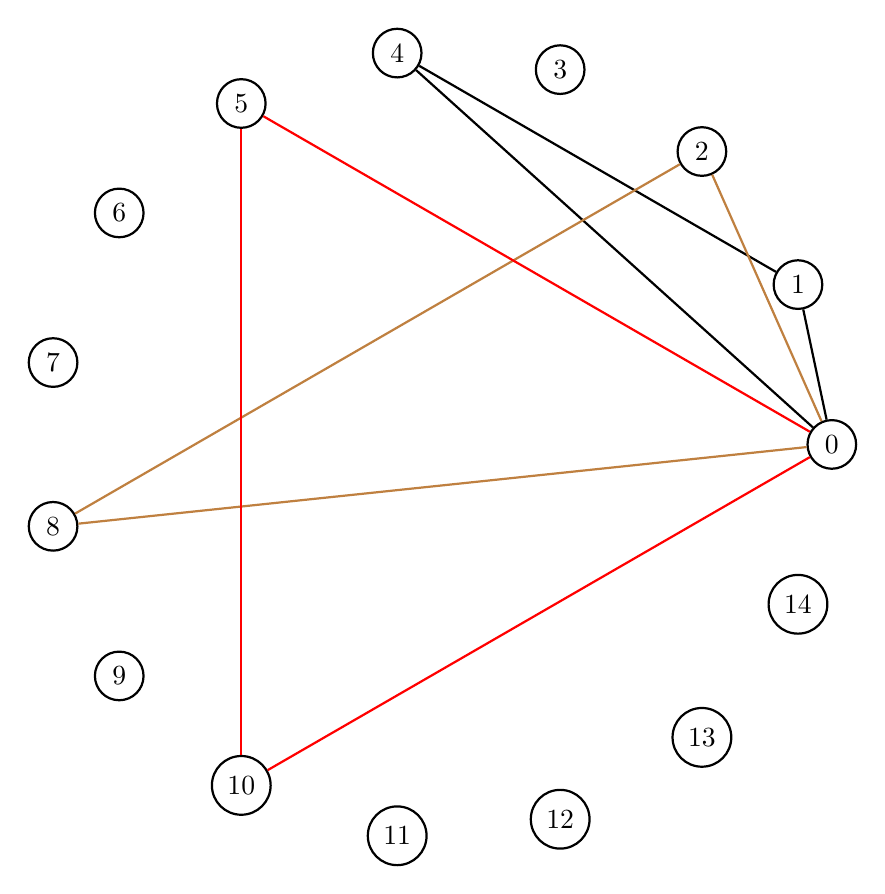
\begin{tikzpicture}
\begin{scope}[every node/.style={circle,thick,draw}]
\node (0) at (5.0, 0.0) {0}; 
\node (1) at (4.57, 2.03) {1}; 
\node (2) at (3.35, 3.72) {2}; 
\node (3) at (1.55, 4.76) {3}; 
\node (4) at (-0.52, 4.97) {4}; 
\node (5) at (-2.5, 4.33) {5}; 
\node (6) at (-4.05, 2.94) {6}; 
\node (7) at (-4.89, 1.04) {7}; 
\node (8) at (-4.89, -1.04) {8}; 
\node (9) at (-4.05, -2.94) {9}; 
\node (10) at (-2.5, -4.33) {10}; 
\node (11) at (-0.52, -4.97) {11}; 
\node (12) at (1.55, -4.76) {12}; 
\node (13) at (3.35, -3.72) {13}; 
\node (14) at (4.57, -2.03) {14}; 
 
\draw[thick, black] (0) -- (1); 
\draw[thick, black] (1) -- (4); 
\draw[thick, black] (0) -- (4); 

\draw[thick, brown] (0) -- (2); 
\draw[thick, brown] (2) -- (8); 
\draw[thick, brown] (0) -- (8); 

\draw[thick, red] (0) -- (5); 
\draw[thick, red] (5) -- (10); 
\draw[thick, red] (0) -- (10); 
\end{scope}
,
\end{tikzpicture}
\caption{s=7, g=3, n=15, m=35, node 0 adjacencies. $i \in [0, 4): (i, i+5, i+10); \forall i: (i, i+1, i+4), (i, i+2, i+8)$, all $\mod 15$}
\label{fig:s7g3}
\end{figure}

Apparently some versions of this problem were studied even in the nineteenth century. Kirkman's schoolgirl problem\cite{5} asks: \emph{Can fifteen girls walk in groups of three to school for seven days, such that each pair walks together exactly once?}. With colors representing walking groups, $s=7, g=3, n=15, m=35$, we have something isomorphic to a Spot It deck construction. 

Through ad-hoc tinkering, we can find the graph in Fig.~\ref{fig:s7g3}, showing the adjacencies for a single node. These are repeated ``round the horn'', with the exception that the red triangle only appears five times instead of 15.

\begin{figure}[!htb]
\centering
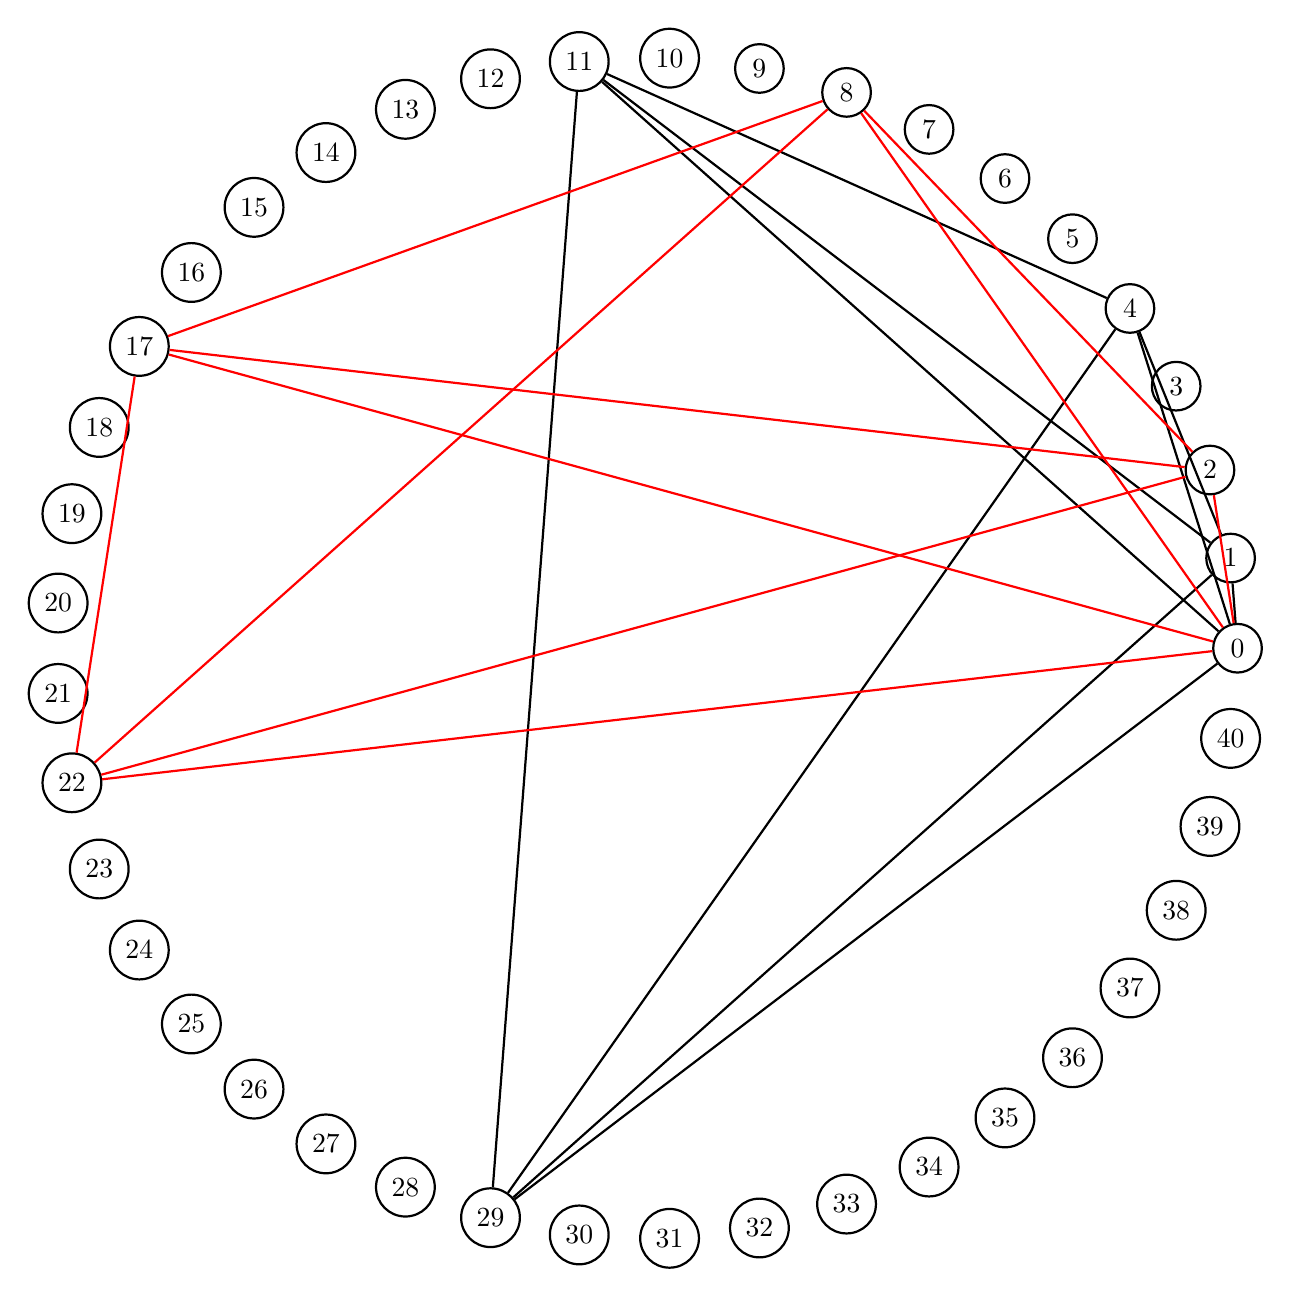
\begin{tikzpicture}
\begin{scope}[every node/.style={circle,thick,draw}]
\node (0) at (7.5,0) {0};
\node (1) at (7.412,1.145) {1};
\node (2) at (7.15,2.263) {2};
\node (3) at (6.721,3.328) {3};
\node (4) at (6.134,4.315) {4};
\node (5) at (5.404,5.201) {5};
\node (6) at (4.547,5.965) {6};
\node (7) at (3.583,6.589) {7};
\node (8) at (2.535,7.059) {8};
\node (9) at (1.428,7.363) {9};
\node (10) at (0.287,7.494) {10};
\node (11) at (-0.86,7.451) {11};
\node (12) at (-1.987,7.232) {12};
\node (13) at (-3.068,6.844) {13};
\node (14) at (-4.077,6.295) {14};
\node (15) at (-4.99,5.599) {15};
\node (16) at (-5.786,4.772) {16};
\node (17) at (-6.447,3.833) {17};
\node (18) at (-6.956,2.804) {18};
\node (19) at (-7.303,1.709) {19};
\node (20) at (-7.478,0.574) {20};
\node (21) at (-7.478,-0.574) {21};
\node (22) at (-7.303,-1.709) {22};
\node (23) at (-6.956,-2.804) {23};
\node (24) at (-6.447,-3.833) {24};
\node (25) at (-5.786,-4.772) {25};
\node (26) at (-4.99,-5.599) {26};
\node (27) at (-4.077,-6.295) {27};
\node (28) at (-3.068,-6.844) {28};
\node (29) at (-1.987,-7.232) {29};
\node (30) at (-0.86,-7.451) {30};
\node (31) at (0.287,-7.494) {31};
\node (32) at (1.428,-7.363) {32};
\node (33) at (2.535,-7.059) {33};
\node (34) at (3.583,-6.589) {34};
\node (35) at (4.547,-5.965) {35};
\node (36) at (5.404,-5.201) {36};
\node (37) at (6.134,-4.315) {37};
\node (38) at (6.721,-3.328) {38};
\node (39) at (7.15,-2.263) {39};
\node (40) at (7.412,-1.145) {40};
 
 (((0 1 4 11 29) (0 2 8 17 22)))
 
\draw[thick, black] (0) -- (1); 
\draw[thick, black] (0) -- (4); 
\draw[thick, black] (0) -- (11); 
\draw[thick, black] (0) -- (29); 

\draw[thick, black] (1) -- (4); 
\draw[thick, black] (1) -- (11); 
\draw[thick, black] (1) -- (29); 

\draw[thick, black] (4) -- (11); 
\draw[thick, black] (4) -- (29); 

\draw[thick, black] (11) -- (29); 


\draw[thick, red] (0) -- (2); 
\draw[thick, red] (0) -- (8); 
\draw[thick, red] (0) -- (17); 
\draw[thick, red] (0) -- (22); 

\draw[thick, red] (2) -- (8); 
\draw[thick, red] (2) -- (17); 
\draw[thick, red] (2) -- (22); 

\draw[thick, red] (8) -- (17); 
\draw[thick, red] (8) -- (22); 

\draw[thick, red] (17) -- (22); 


\end{scope}
,
\end{tikzpicture}
\caption{Perfect Difference Set on s=10, g=5, n=41, m=82: (0 1 4 11 29), (0 2 8 17 22)}
\label{fig:s10g5}
\end{figure}

These are apparently instances of a \emph{Steiner Triple System} $S(t, k, n)$\cite{6}, where we look for groups of $k$ among $n$ total elements, which cover exactly once every set of size $t$. If $t=2$ (edges in the graph, pairs of girls), and $k=3$ (subgroups $K_3$, walking trios) among $n$, we have an instance of a Kirkman problem (and Spot It game); in fact, Kirkman problems are those where $t=2, k=3$.

The followups to this problem are varied (including links to projective and affine geometry) and many unsolved ($t \geq 6$). Much progress has been made on $STS(t=2,k=3,n)$ but results seem spotty for $k>3$.

By some backtracking and brute force searching using our code \url{https://github.com/fettermania/mathnotes/tree/main/spotit/code}, we can find a few ad-hoc solutions on our own, even without the problem fully solved:



\begin{figure}[!htb]
\centering
 \centering
 \begin{tabular}{c c | c | c }
 s & g & adjacencies $\forall i$ & adjacencies $i \in [0, g-1]$ \\
\hline
 6 & 3 & \{\{0 1, 4\}, \{0, 2, 7\}\} & \{\}\\
 7 & 3 & \{\{0 1 3\}, \{0, 4, 10\}\} & \{\{0, 5, 10\}\} \\
 9 & 3 & \{\{0,1,6\}, \{0,2,10\}, \{0,3,7\} & \{\} \\
 10 & 3 & \{\{0,2,10\}, \{0,1,5\}, \{0,3,9\}\} & \{\{0, 7, 14\}\} \\
 10 & 5 & \{\{0, 1, 4, 11, 29\}, \{0, 2, 8, 17, 22\}\} & \{\} \\
 \end{tabular}
 \caption{Ad Hoc Steiner Solutions }
\label{fig:ad-hoc-steiner}
\end{figure}

The adjacencies for node 0 in $s=10, g=5$ are shown in Fig.~\ref{fig:s10g5}, obtained through computational means.

\section{Nonuniform g: deletion and partial inception}

All of our solutions were concerned with a Spot It deck in which every symbol appears exactly $g$ times. The commercial deck has $s=8$ on all cards, but contains $n=55$ cards instead of $s(g-1) +1 = 8(7) = 57$ cards, assuming $g=8$. The most likely explanation is that two cards were simply deleted. Deletion from a deck created with the methods above yields a deck in which $s$ remains constant but $g$ can vary. This could also occur if we replaced \emph{some} of the complete subgraphs $K_g$ with ``incepted'' graphs (section 8). It's also likely that we could greedily construct a deck with consistent $s$ if we were unconcerned if $g$ were uniform across colors.

\section{Open questions}

In addition to the many open questions in Steiner Systems\cite{6}, which would include the whether any $g | s$ or $g | s-1$ has a solution, we have other questions about our systems:

\begin{itemize}
\item For an it be true that $g | s(s-1)$ but not true that $g | s$ or $g | s-1$ (e.g. $g=6, s=9$)?
\item Are all constructions where $g=s-1$ isomorphic?
\end{itemize}



\begin{thebibliography}{9}
\bibitem{1} Singer, James. ``A THEOREM IN FINITE PROTECTIVE GEOMETRY AND SOME APPLICATIONS TO NUMBER THEORY'', 1934. \url{https://www.ams.org/journals/tran/1938-043-03/S0002-9947-1938-1501951-4/S0002-9947-1938-1501951-4.pdf} 
\bibitem{2} ``The Mind-Bending Math Behind Spot It!, the Beloved Family Card Game'', Smithsonian Magazine. \url{https://www.smithsonianmag.com/science-nature/math-card-game-spot-it-180970873/}
\bibitem{3} Wikipedia: {https://en.wikipedia.org/wiki/Graph\_partition}
\bibitem{4} Adleman, Leonard M. and Lenstra, Hendrik W. ``FINDING IRREDUCIBLE POLYNOMIALS OVER FINITE FIELDS'' \url{https://www.math.leidenuniv.nl/~hwl/PUBLICATIONS/1986a/art.pdf}
\bibitem{5} Wikipedia: \url{https://en.m.wikipedia.org/wiki/Kirkman\%27s_schoolgirl_problem}
\bibitem{6} Wikipedia: \url{https://en.wikipedia.org/wiki/Steiner_system}
\end{thebibliography}


\end{document}


